%%% Local Variables:
%%% mode: latex
%%% TeX-master: "../report"
%%% End:

\subsection{Definition of terms}
\begin{description}
\item[Compiler] \hfill \\
  A program that translates (potentially high-level) program code into
  another language. Common targets are assembly languages for either
  hardware CPUs or abstract machines. Examples include
  \texttt{gcc}\cite{NEEDED}, \texttt{javac}\cite{NEEDED} and
  \texttt{ghc}\cite{NEEDED}.

\item[Object-Orientation] \hfill \\
  Foo bar

\item[Intermediate Language (or Intermediate Representation)] \hfill \\
  TODO

\item[C Macro] \hfill \\
  A macro in GCC is essentially a named code fragment. The C
  preprocessor\footnote{The C Preprocessor - GCC - Gnu:
    \url{https://gcc.gnu.org/onlinedocs/cpp/}} inserts the fragment
  wherever the name is used. A macro can also take arguments, where
  the given argument will be inserted where ever it used in the
  fragment. For more information, see the GCC documentation
  \url{https://gcc.gnu.org/onlinedocs/cpp/Macros.html}.

\item[Mock Object] \hfill \\
  A mock object is a simulated object which mimics the behavior of the
  actual object. This is useful for testing, as the programmer can
  mock different states of an object and return test the result of
  different procedures or functions. % TODO: avoid plagiarism

\end{description}


% \subsection{\thename{} Specification}
\label{sec:spec}
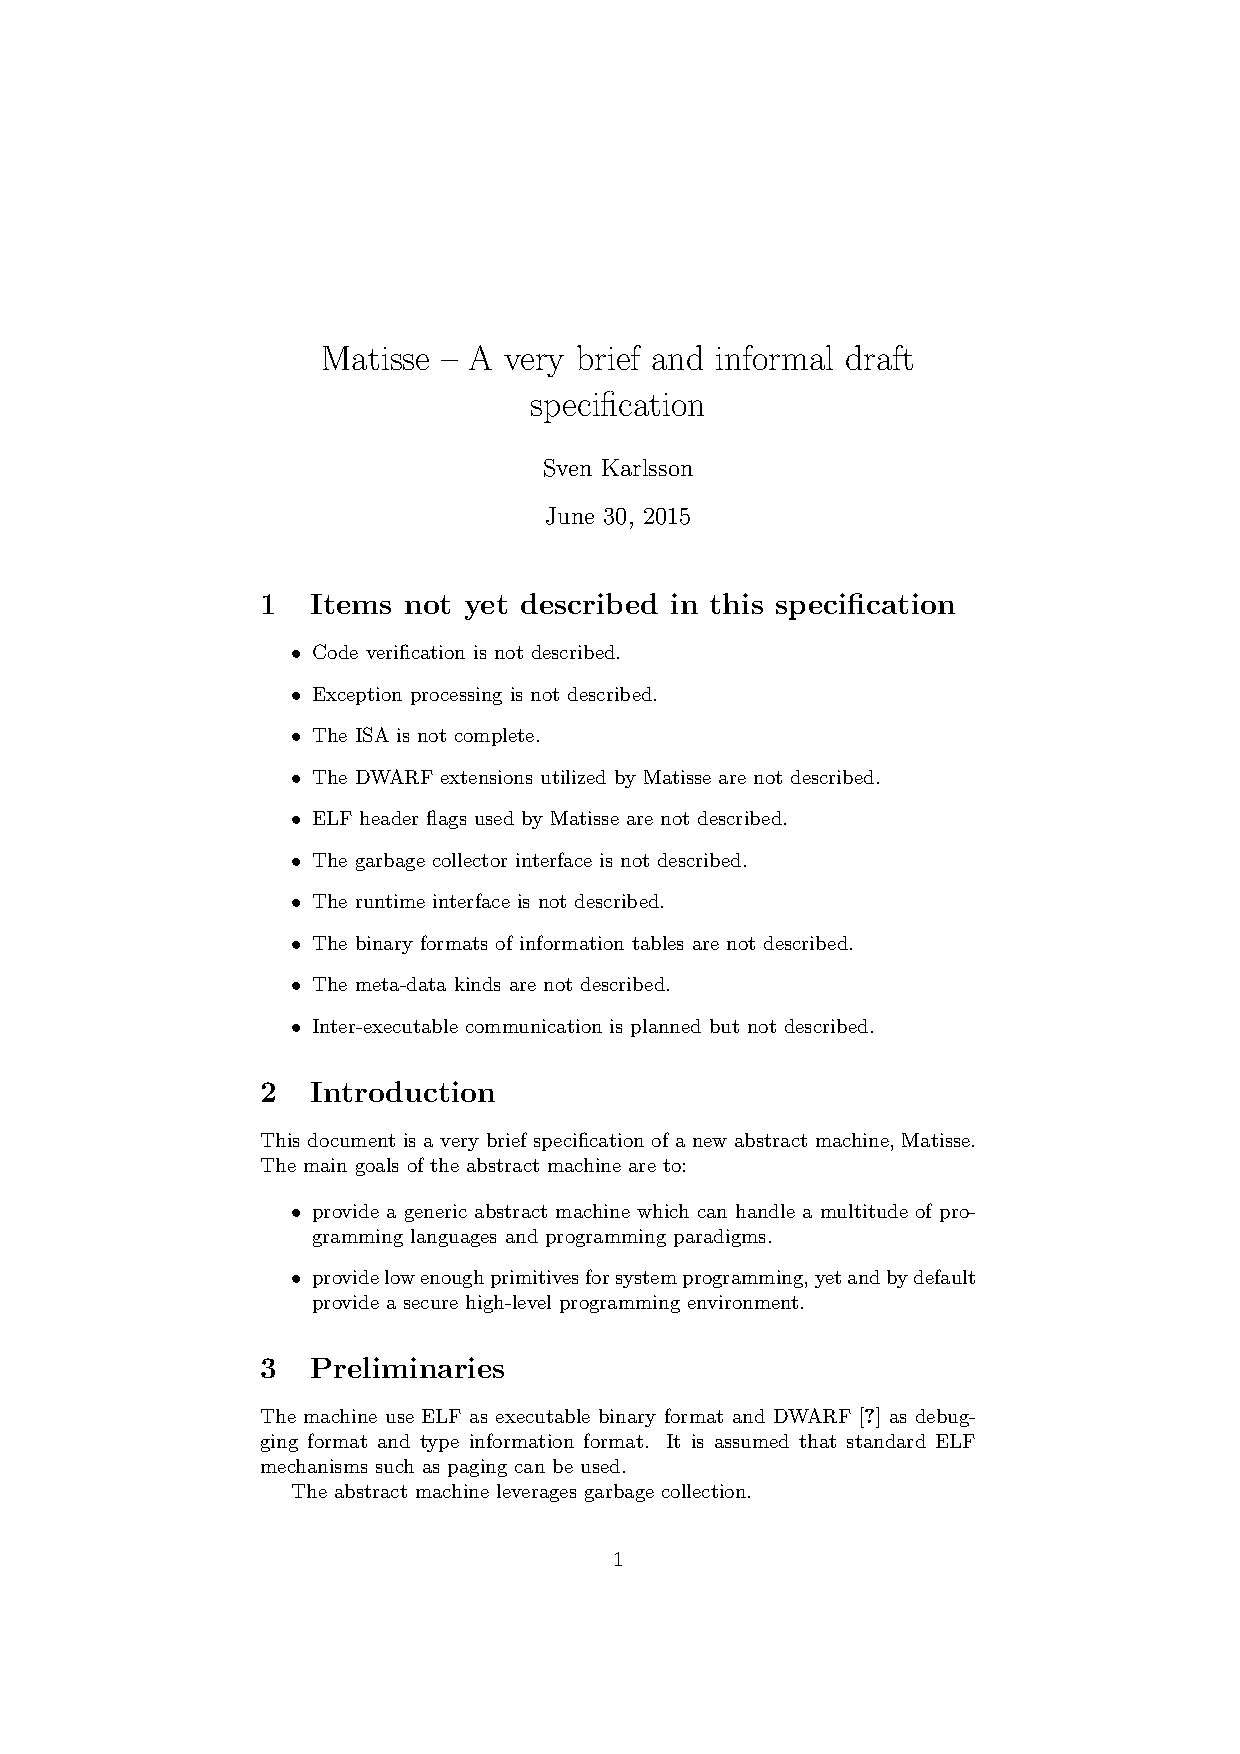
\includepdf[pages=-]{lib/spec.pdf}
